\documentclass[tikz,border=8pt]{standalone}
\usepackage[utf8]{inputenc}
\usepackage[OT4,plmath]{polski}
\usepackage{amsmath,amssymb}
\usetikzlibrary{patterns}
\begin{document}
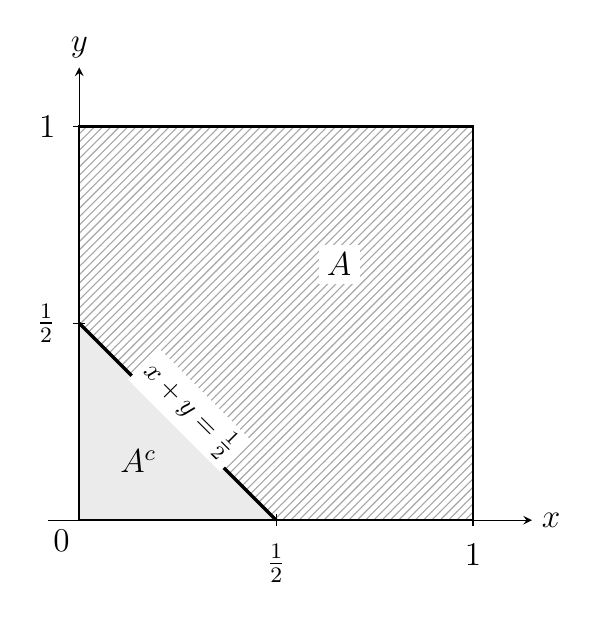
\begin{tikzpicture}[x=5cm,y=5cm,>=stealth,font=\large]
  \fill[pattern=north east lines,pattern color=black!35]
    (0,.5)--(0,1)--(1,1)--(1,0)--(.5,0)--cycle;
  \fill[black!8] (0,0)--(.5,0)--(0,.5)--cycle;
  \draw[thick] (0,0) rectangle (1,1);
  \draw[very thick] (0,.5)--(.5,0);
  \draw[->] (-.08,0)--(1.15,0) node[right] {$x$};
  \draw[->] (0,0)--(0,1.15) node[above] {$y$};
  \foreach \x/\lab in {.5/{\frac12},1/{1}} {
    \draw (\x,.015)--(\x,-.015) node[below=3pt] {$\lab$};
  }
  \foreach \y/\lab in {.5/{\frac12},1/{1}} {
    \draw (.015,\y)--(-.015,\y) node[left=3pt] {$\lab$};
  }
  \node[below left] at (0,0) {$0$};
  \node[fill=white,inner sep=3pt] at (.66,.65) {$A$};
  \node at (.15,.15) {$A^c$};
  \node[fill=white,inner sep=2pt,rotate=-45,font=\normalsize]
    at (.28,.28) {$x+y=\frac12$};
\end{tikzpicture}
\end{document}
